%TCIDATA{LaTeXparent=0,0,RUL1.tex}

\begin{biography}[{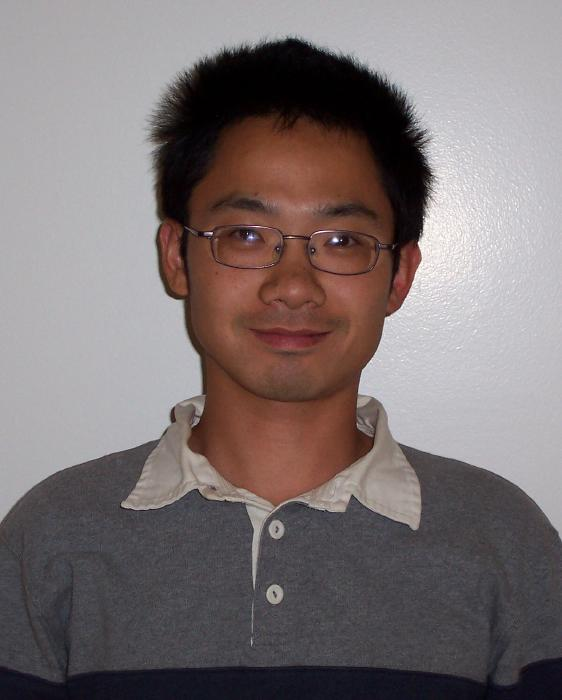
\includegraphics[width=1in,height=1.25in,clip]{BioPhotos/shufang.jpg}}]{Shufang Dong}
earned his Bachelor of Science from Beijing Institute of Technology in 1994 and Master of Science in Mechanical Engineering from Shanghai Jiaotong University in 1997, China. He worked for the United Automotive Electronics System Company in Shanghai as an injection molding engineer, and product and equipment engineer specializing automatic engine management systems until he came to the University of Delaware in 2001. Now he is a Ph.D. candidate in the Department of Mechanical Engineering with research interests in physical rehabilitation devices, biomechanics of human movement, smart fluids and applied nonlinear control.
\end{biography}

\begin{biography}[{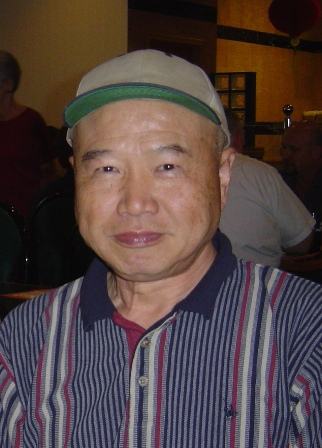
\includegraphics[width=1in,height=1.25in,clip]{BioPhotos/kql.jpg}}]{Ke-Qian Lu}
was a professor of Measurement and Electronic Engineering in Tianjin University, China. 
He has been a researcher in the Department of Mechanical Engineering at the University of Delaware since 2001.
\end{biography}


\begin{biography}[{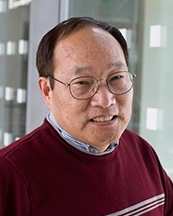
\includegraphics[width=1in,height=1.25in,clip]{BioPhotos/jqs.jpg}}]{J.Q. Sun}
earned his PhD from University of California at Berkeley in 1988.  He worked for Lord Corporation at their Corporate R\&D Center in Cary, North Carolina, and since engaged in smart materials research and applications, and acoustic-structural controls.  In 1994, Dr. Sun joined the faculty of the department of Mechanical Engineering at the University of Delaware as an Assistant Professor, was promoted to Associate Professor in 1998 and to Professor in 2003.  He was an Associated Editor of ASME Journal of Vibration and Acoustics since 1994 to 2000, and has been an Associated Editor of Communications in Nonlinear Science and Numerical Simulations since 2001 and an Editorial Member of Acta Mechanica Solida Sinica since 2003.  His research interests include nonlinear random vibrations, nonlinear controls, active structural-acoustic control, modeling and application of smart materials.
\end{biography}

\begin{biography}[{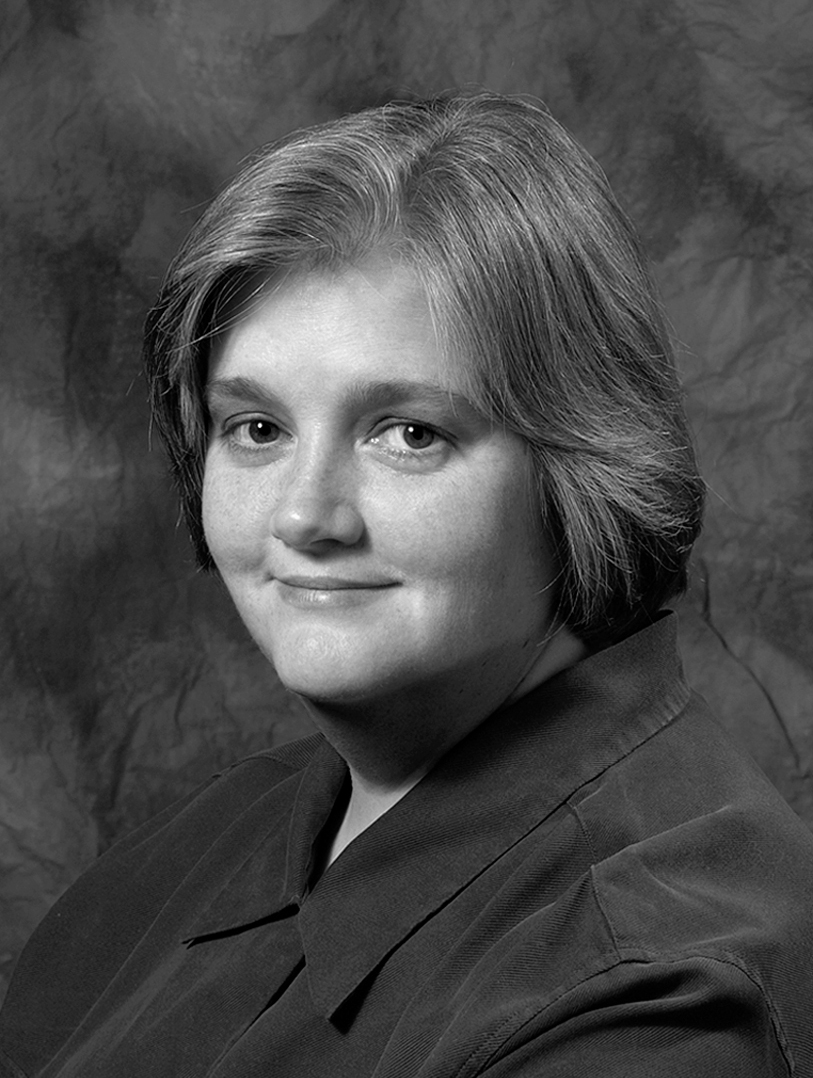
\includegraphics[width=1in,height=1.25in,clip]{BioPhotos/kr.jpg}}]{Katherine Rudolph}
earned her Master of Science in Physical Therapy from Boston University in 1989 and her PhD in Biomechanics and Movement Sciences from the University of Delaware in 1998.  Dr. Rudolph joined the faculty of the Department of Physical Therapy and Program in Biomechanics and Movement Sciences at the University of Delaware in 1999 and is currently an Assistant Professor.  She has served as a manuscript reviewer for the Journal of Orthopaedic and Sports Physical Therapy, Archives of Physical Medicine and Rehabilitation, Journal of Applied Biomechanics and the European Journal of Applied Physiology and has reviewed grants for the National Institutes of Health Musculoskeletal and Rehabilitation Sciences Study section. Dr. Rudolph's research interests include analysis of walking in patients with knee osteoarthritis and neurological injury and development of research based physical therapy interventions.
\end{biography}

